\Chapter{}
\chapter{METODOLOGÍA}
    \section{Área de estudio (unidad de análisis)}
        La investigación inicialmente se enfocó en la armonización y superresolución de imágenes Landsat MSS y TM de diversas regiones a nivel mundial, excluyendo la Antártida por su homogeneidad espectral, principalmente dominada por extensas áreas de hielo y nieve, lo que dificulta la diferenciación de coberturas y complica la armonización satelital \autocite{kokhanovsky2019retrieval}. De forma similar, se descartaron las regiones oceánicas debido a su uniformidad espectral, lo que limita la variabilidad en la reflectancia \autocite{estrella2021spectral}. En consecuencia, el estudio se centró en áreas continentales no homogéneas en términos de reflectancia.
        \begin{figure}[H] 
            \caption{\doublespacing \\ \textit{Mapa del área de estudio.}} 
            \centering
            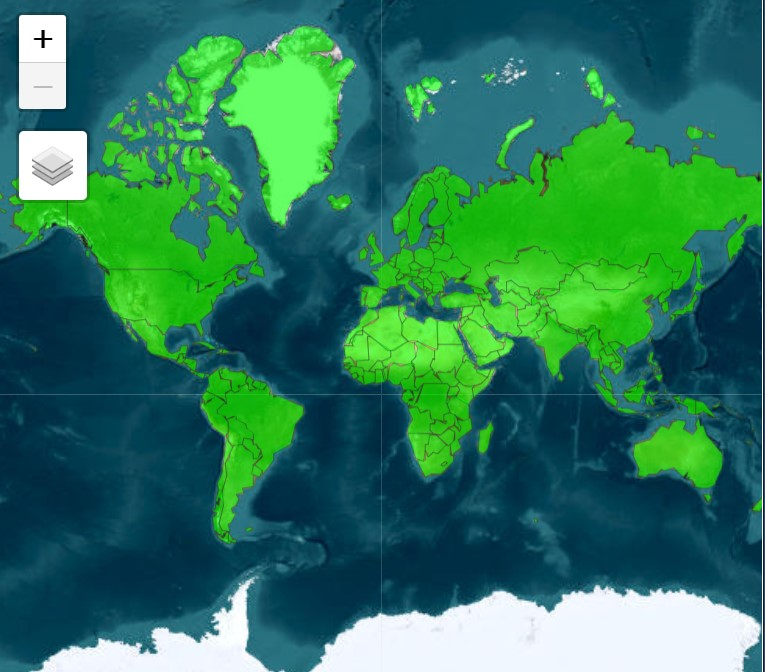
\includegraphics[width=1\linewidth]{E_IMAGENES/area_estudio.jpg}
            \begin{justify}
                \textit{Nota.} Se muestra un mapa satelital global, resaltando las zonas terrestres verdes, omitiendo océanos y la Antártida.
            \end{justify}                    
            \label{area_estudio}
        \end{figure}

        En la siguiente fase del estudio, se seleccionó estratégicamente Perú como área de la aplicación del autocompletado de bandas o canales que le faltan a las imágenes MSS para parecerse espectralmente a las TM. Esta elección se justifica por la variada topografía y diversidad de ecosistemas del país, que van desde la costa del Pacífico hasta las alturas de los Andes, ofreciendo un escenario desafiante y representativo para la superresolución satelital. Se identificaron múltiples puntos de muestreo distribuidos a lo largo del país, en los cuales se extrajeron segmentos de imágenes MSS para su transformación a la resolución de imágenes TM. 

        \begin{figure}[H] 
            \caption{\doublespacing \\ \textit{Mapa del área para la validación de los modelos.}} 
            \centering
            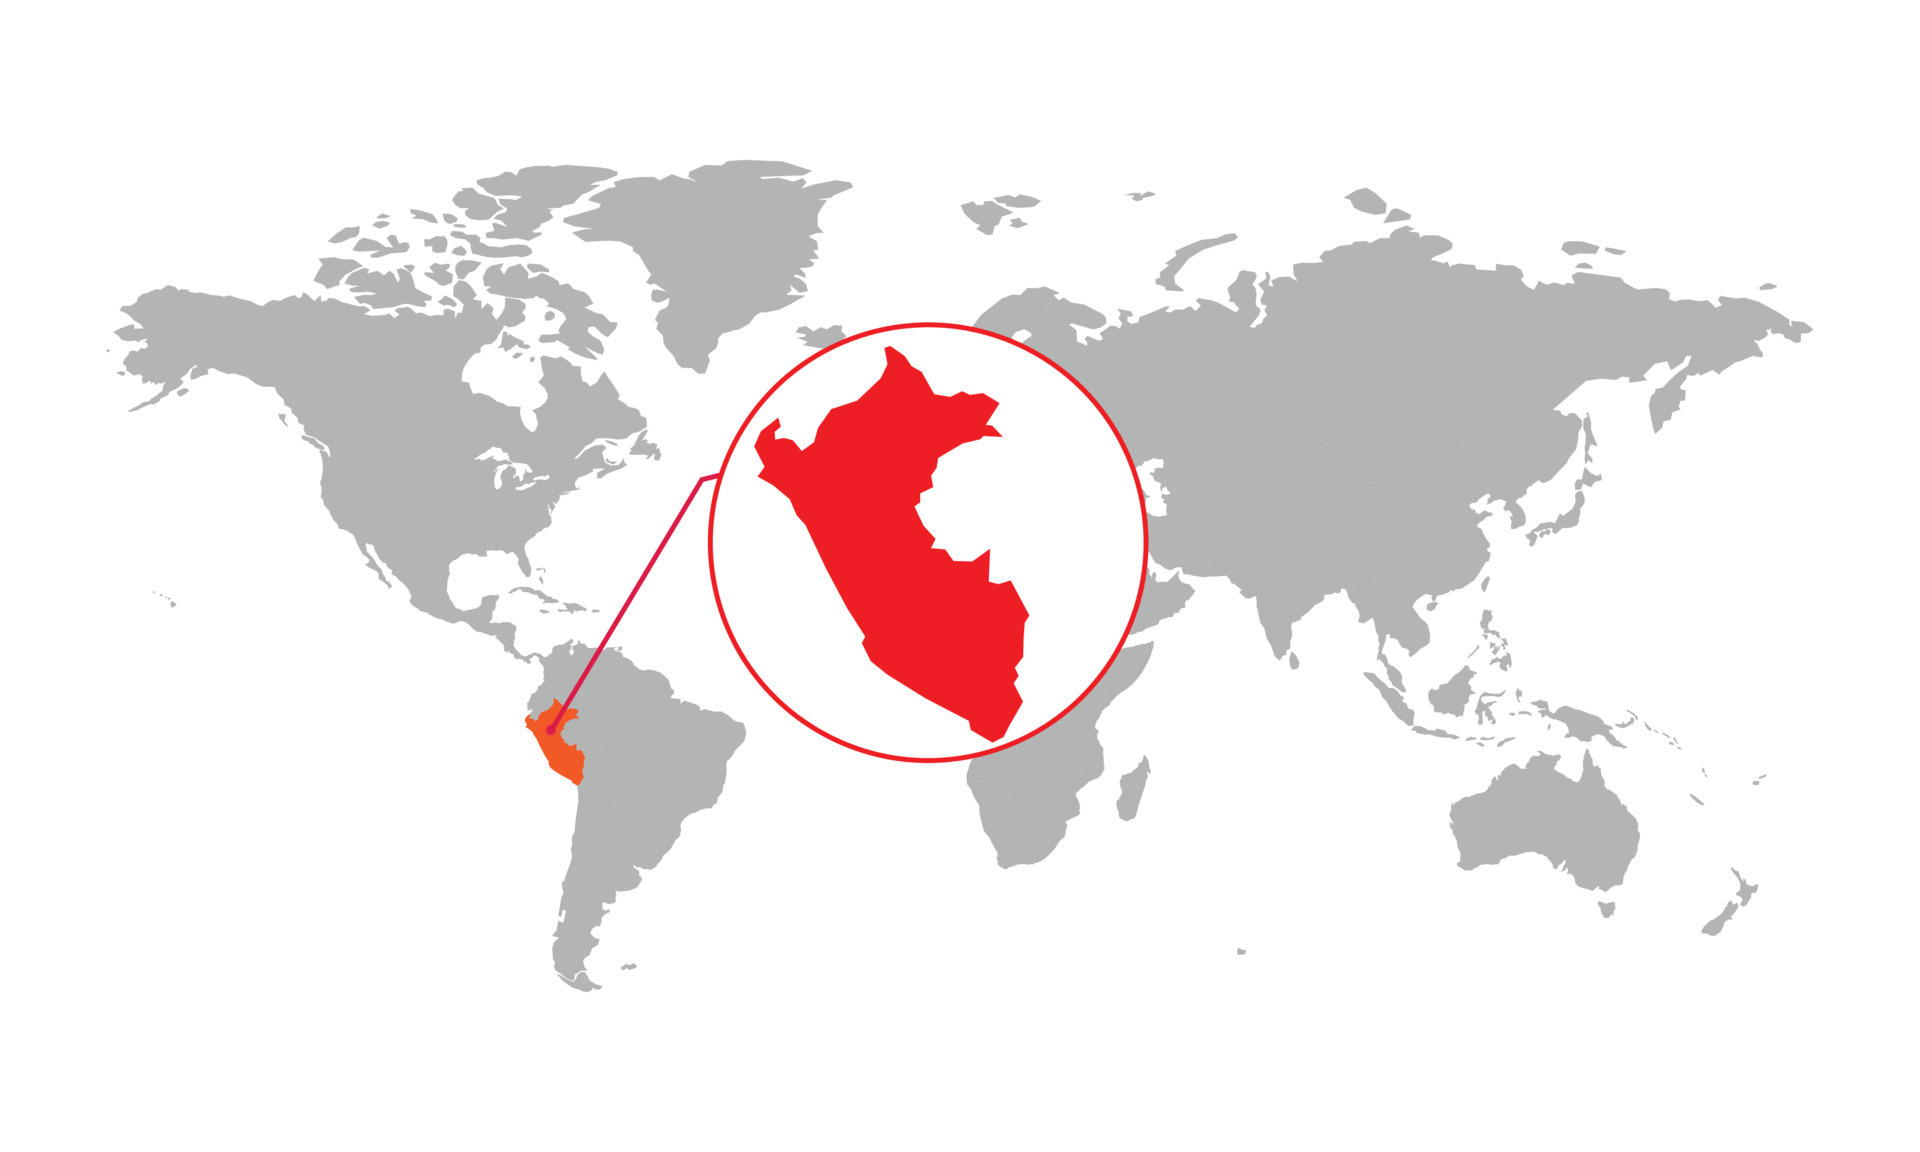
\includegraphics[width=0.8\linewidth]{2_CAPITULO4/IMG/mapa_peru.jpg}
            \begin{justify}
                \textit{Nota.} Se muestra un mapa de Perú, teniendo en cuenta toda su área, por su diversidad ecosistémica.
            \end{justify}                    
            \label{peru}
        \end{figure}

    \section{Diseño de investigación}
        En el marco del diseño de investigación de la tesis que aborda la armonización de imágenes Landsat MSS mediante inteligencia artificial, se adoptan criterios metodológicos que se alinean con los planteamientos de (Sampieri, 2018). Esta estructura metodológica se desglosa en las siguientes categorías:
        %\autocite{sampieri2018metodologia}
        \subsection{Tipo}
            La investigación se clasifica como aplicada, ya que tiene el objetivo de resolver problemas específicos relacionados con la armonización de imágenes satelitales, aplicando teorías y conocimientos de inteligencia artificial. Este tipo de investigación busca generar soluciones prácticas que puedan ser implementadas en el ámbito del monitoreo global y a largo plazo.

        \subsection{Nivel}
            Corresponde al nivel descriptivo, ya que se centra en describir las características y el comportamiento de un fenómeno o realidad específica, en este caso, la capacidad de la inteligencia artificial para mejorar la armonización de las imágenes Landsat MSS. A través de este nivel, se busca detallar las particularidades, diferencias o modalidades de un fenómeno sin ejercer control sobre las variables de estudio.

        \subsection{Enfoque}
            El enfoque de la investigación es cuantitativo, dado que se recopilan y analizan datos numéricos para evaluar la eficacia de los métodos de inteligencia artificial en la armonización de imágenes. Este enfoque permite una medición objetiva y estadística de los resultados, facilitando la comparación y el análisis de la efectividad de las técnicas empleadas.  

	    \subsection{Diseño}
            El diseño de esta investigación es no experimental, transeccional o transversal descriptivo. Esto significa que se observan fenómenos tal como se dan en su contexto natural para luego describirlos, sin manipular las variables de estudio. En este caso, se analiza la efectividad de la inteligencia artificial en la armonización de imágenes Landsat MSS, evaluando los datos existentes en un único momento, o en varios momentos bajo el mismo criterio, sin intervenir o modificar las condiciones bajo las cuales se obtuvieron dichas imágenes.

         
    \section{Población y muestra}
    
        \subsection{Población}
            La población de este estudio incluye imágenes capturadas por los sensores MSS y TM de los satélites Landsat 4 y 5, enfocándose en regiones continentales globales, excluyendo la Antártida y zonas oceánicas, entre 1982 y 1999. Estas imágenes, accesibles a través de las bases de datos de Landsat, ofrecen un registro histórico integral para la extracción de datos necesarios en esta investigación, permitiendo analizar las características y cambios en las regiones seleccionadas durante el periodo especificado.
            

        \subsection{Muestra}
            El enfoque de muestreo implementado es probabilístico, lo cual implica la selección aleatoria de unidades de muestreo para asegurar la independencia estadística y representatividad de las imágenes MSS y TM de Landsat en la muestra. Estas imágenes son elegidas basándose en criterios específicos, incluyendo un intervalo de tiempo de captura menor a 10 minutos entre ellas y una cobertura de nubosidad inferior al 15 \%, además de cumplir con requisitos de concordancia espacial. Siguiendo los lineamientos propuestos por \textcite{hernandez2014recoleccion} sobre recolección de datos, se ha establecido un tamaño de muestra de 5431 pares de imágenes. Esta cifra refleja adecuadamente la totalidad de la población estudiada, garantizando un análisis robusto y representativo de los datos.
            
    \section{Procedimiento, técnicas e instrumentos de recolección de información}

       \subsection{Obtención de datos de entrada}
            \subsubsection{Selección por localización}
                Para garantizar la eficacia y precisión de la investigación, se llevó a cabo una meticulosa selección de imágenes para el estudio. A continuación, se detalla el procedimiento de selección:
                
                \begin{enumerate}
                    \item Como punto de partida, se generaron puntos de manera aleatoria alrededor del mundo, resultando en un total inicial de 20 000 puntos. Estos puntos sirvieron como centroides para definir buffers cuadrados con dimensiones de 30 720 metros por lado.
                    
                    \begin{figure}[H] 
                        \caption{\doublespacing \\ \textit{Generación de 20 000 puntos aleatorios a nivel mundial.}} 
                        \centering
                        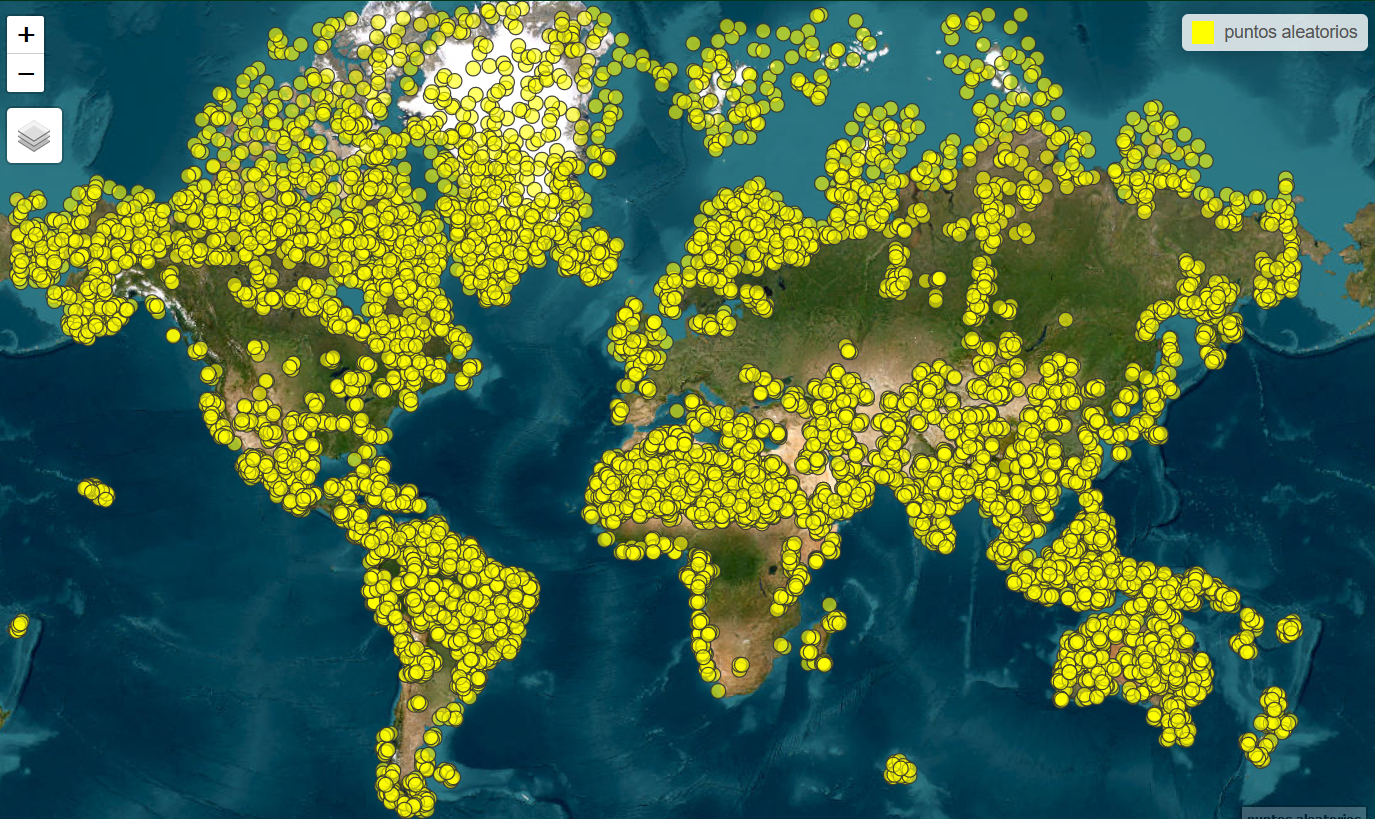
\includegraphics[width=0.9\linewidth]{2_CAPITULO0/IMG/1000points.png}
                        \begin{justify}
                            \textit{Nota.} Los puntos no excedieron los límites del WRS-2 (desde Landsat 4 hasta Landsat 9), que corresponden a las áreas o segmentos de captura de todas las imágenes Landsat, incluyendo los sensores más recientes.
                        \end{justify}                    
                        \label{1000points}
                    \end{figure}

        
                    \item Con los puntos geográficos establecidos, se procedió a seleccionar imágenes específicas. Se optó por imágenes MSS pertenecientes exclusivamente a las misiones Landsat 4 y 5, ya que coinciden con las imágenes obtenidas por el sensor TM de las mismas misiones durante el período de 1982 a 1999.
                
                    \item Una condición crucial en esta fase fue asegurar que el área definida por cada buffer estuviera íntegramente contenida dentro de al menos una imagen MSS y una imagen TM. Este criterio busca prevenir truncamientos o limitaciones en la amplitud de las imágenes.
                    
                    \item Se excluyeron ciertas áreas geográficas del proceso: específicamente, regiones de la Antártida y zonas mayormente oceánicas, para asegurar la relevancia y calidad del conjunto de datos final.
                    
                    \item Tras aplicar todos los criterios anteriores, de los 20 000 puntos iniciales, solo 19 546 satisfacían todas las condiciones y, por lo tanto, fueron retenidos para el estudio.
                \end{enumerate}
            \subsubsection{Selección por tiempo y calidad}
                Tras el filtro geográfico inicial, se procedió a una selección más detallada basada en criterios temporales y de calidad. A continuación se describe el procedimiento adoptado:
                
                \begin{enumerate}
                    \item De los 20 000 puntos iniciales, solo 19 546 cumplían con los criterios de localización. Para estos puntos seleccionados, se llevó a cabo una comparación temporal entre las imágenes de ambos sensores.
                
                    \item La condición impuesta fue que las imágenes de ambos sensores debían tener un diferencial temporal no superior a 10 minutos. Es decir, por cada punto, se retuvieron solo aquellos pares que hubieran sido capturadas en un intervalo de tiempo menor o igual a 10 minutos entre ellas.
                    
                    \item Es importante mencionar que este filtro temporal se aplicó considerando imágenes de los niveles Tier 1 y Tier 2 para ambos sensores. Debido a este riguroso criterio, no todos los puntos conservaron la misma cantidad de imágenes, y algunos incluso quedaron sin imágenes que cumplieran con este requisito.
                    
                    \item Posterior al filtro temporal, se implementó un filtro de calidad basado en la nubosidad. Se utilizó la banda de calidad (QA), específicamente de las imágenes del sensor TM, para evaluar la presencia de nubes o sombras. El criterio adoptado fue que las imágenes retenidas no debieran tener una cobertura de nubes o sombras que superara el 15\% del área del buffer generado por el punto dentro de la extensión de la imagen.
                    
                    \item Al concluir estos filtros, se obtuvo un conjunto final de imágenes (15 878 pares) filtradas que satisfacen tanto los criterios de diferencial temporal como los de calidad en relación con la nubosidad.
                \end{enumerate}
                
                Este enfoque garantizó un conjunto de datos con alta precisión temporal y calidad visual, minimizando las distorsiones o interferencias potenciales debido a la nubosidad.

                \begin{figure}[H] 
                    \caption{\doublespacing \\ \textit{Aplicación del algoritmo Fmask en imágenes TM para enmascarar nubes y reducir su interferencia en menos del 15\%.}} 
                    \centering
                    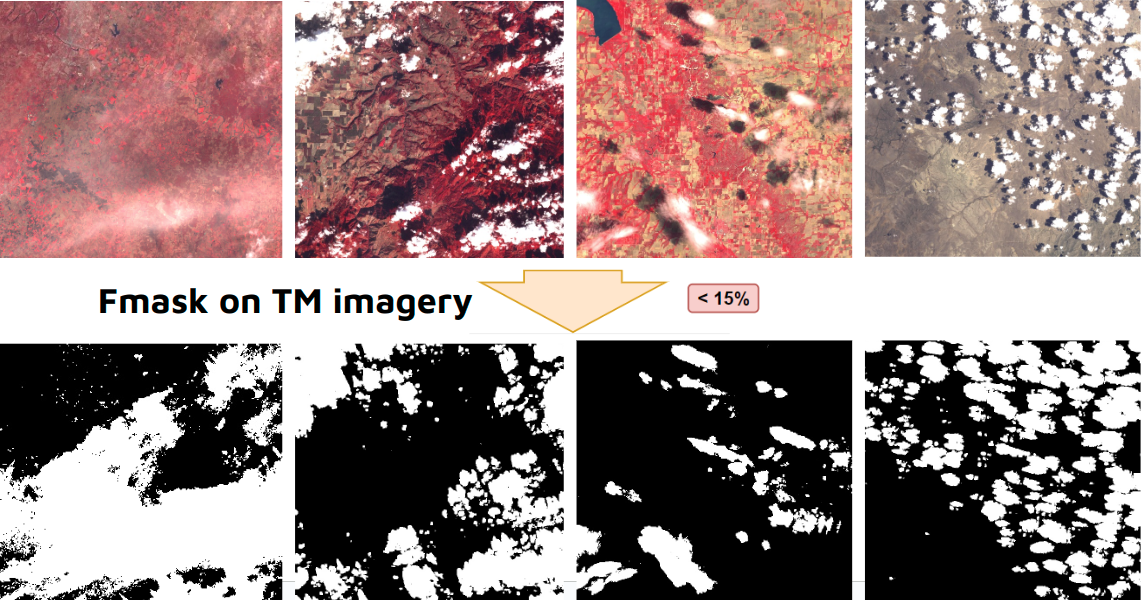
\includegraphics[width=1\linewidth]{2_CAPITULO4/IMG/fmask.png}
                    \begin{justify}
                        \textit{Nota.} El filtrado por nube es una etapa crítica en el procesamiento de imágenes satelitales, se utilizó el algoritmo Fmask para identificar y enmascarar nubes en imágenes de TM (Thematic Mapper), este proceso permite reducir la interferencia de nubes en menos del 15\%, mejorando la calidad de los datos utilizados para análisis posteriores.
                    \end{justify}                    
                    \label{fmask}
                \end{figure}
  
        \subsection{Corrección geométrica de las imágenes MSS}
            El propósito de este proceso es asegurar una alineación precisa entre las imágenes MSS y TM. A continuación, se detallan las etapas de la corrección geométrica:
            
            \subsubsection{Lectura y preprocesamiento de imágenes}
                Se cargan las imágenes, y son normalizadas para tener valores reales de reflectancia. Se seleccionan únicamente las bandas que coinciden entre las imágenes, garantizando su comparabilidad.
            
            \subsubsection{Extracción y coincidencia de características}
                Con la ayuda de modelos de aprendizaje profundo como LightGlue, se identifican puntos clave en ambas imágenes. Estos puntos son luego emparejados para determinar la desalineación entre las imágenes MSS y TM.
                
                \begin{figure}[H] 
                    \caption{\doublespacing \\ \textit{LightGlue: Emparejamiento de Características en Imágenes con Mecanismo Adaptativo.}} 
                    \centering
                    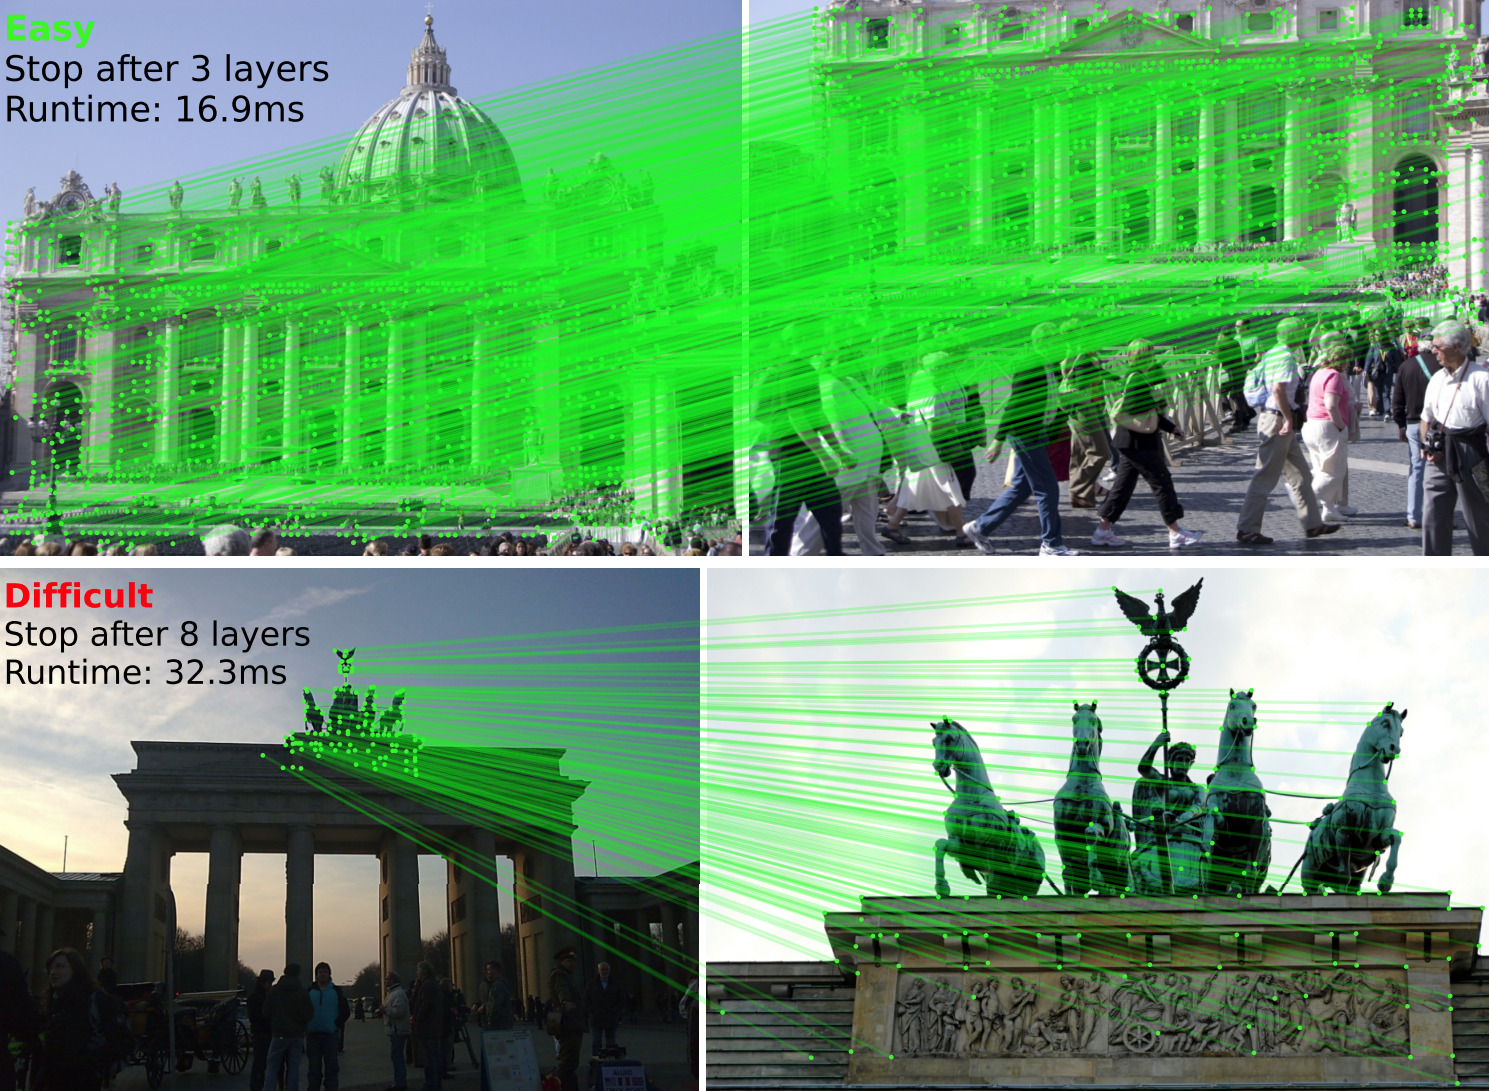
\includegraphics[width=1\linewidth]{2_CAPITULO0/IMG/cvg.png}
                    \begin{justify}
                        \textit{Nota.} La interfaz de 'LightGlue' exhibe dos ejemplos: uno 'fácil' con características emparejadas del Vaticano en 16.9ms y tres capas de procesamiento, y otro "difícil" de un monumento con estatuas, procesado en 32.3ms y ocho capas. Obtenido de \textcite{LightGlue2023}.
                    \end{justify}                    
                    \label{cvg}
                \end{figure}
                
            \subsubsection{Eliminacón de errores calidad y la usabilidad de las MSS}
                En las ímagenes MSS se mostraron errores de líneas saturadas y datos faltantes. Gracias a esta correción se eliminó estos errores, descartando los pares que presentaron estos problemas.

                \begin{figure}[H] 
                    \caption{\doublespacing \\ \textit{Imágenes MSS eliminados por errores del sensor.}} 
                    \centering
                    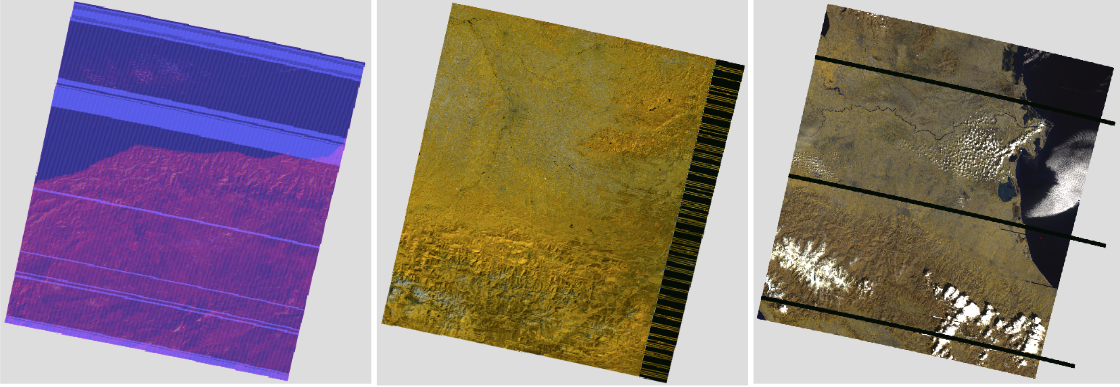
\includegraphics[width=1\linewidth]{2_CAPITULO4/IMG/mss_errores.png}
                    \begin{justify}
                        \textit{Nota.} Corrección geométrica aplicada a imágenes MSS, eliminando errores que afectan la coincidencia con imágenes TM.
                    \end{justify}                    
                    \label{errores_mss}
                \end{figure}

            \subsubsection{Determinación del desplazamiento espacial}
                Usando los puntos clave coincidentes, se estima el desplazamiento espacial entre las imágenes. Este desplazamiento señala cuánto y cómo se desalinean las imágenes en términos de píxeles.

                \begin{figure}[H] 
                    \caption{\doublespacing \\ \textit{Emparejamiento adaptativo de características con LightGlue: De alta resolución (HR) a baja resolución (LR).}} 
                    \centering
                    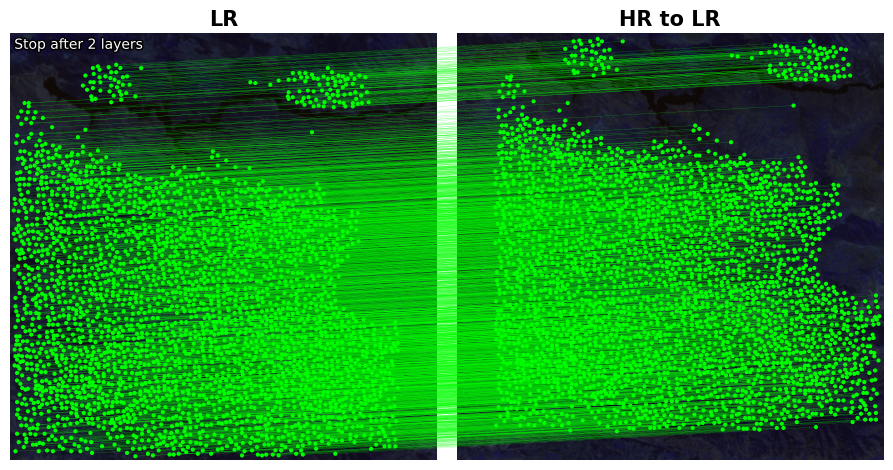
\includegraphics[width=1\linewidth]{2_CAPITULO0/IMG/hr_to_lr.png}
                    \begin{justify}
                        \textit{Nota.} Se observan superposiciones verdes de características detectadas, deteniéndose en ambas tras dos capas, evidenciando la eficacia de "LightGlue".
                    \end{justify}                    
                    \label{hr_to_lr}
                \end{figure}
                
            \subsubsection{Refinamiento subpíxel y convolución en 2D}
                Para refinar la corrección, se recurre a la transformada de Fourier. Esta técnica, mediante la función de correlación cruzada en el dominio de frecuencia, equivale a una convolución en 2D en el dominio espacial. La convolución en 2D es una operación que toma dos imágenes de entrada y produce una tercera imagen como salida, siendo una técnica fundamental en procesamiento de imágenes para filtrar y enfocar. Aquí, ayuda a identificar desplazamientos subpíxeles basados en el contenido de frecuencia de las imágenes.
                
                \begin{equation}
                    X(f) = \int_{-\infty}^{\infty} x(t) \cdot e^{-j2\pi ft} dt
                \end{equation}
            
                Donde \(X(f)\) es la transformada de Fourier de la señal \(x(t)\).
                
                
                Con base en el desplazamiento determinado y su refinamiento subpíxel, las imágenes MSS son alineadas geométricamente con las TM.
                
                Las imágenes MSS corregidas se presentan junto con las TM para confirmar visualmente la alineación. A través del proceso de corrección, se observa una mejora notable en la alineación, evidenciada por la reducción del desajuste visual entre las imágenes. Esta mejora se logra mediante correcciones tanto a nivel de píxel como subpíxel, lo que resulta en una superposición más precisa entre las imágenes MSS y TM.
                
                
                
            \subsubsection{Filtro final de los pares de imágenes}
                En complemento a las técnicas previamente descritas, se incorpora un criterio adicional para la exclusión de correspondencias erróneas entre las imágenes. Se establece un umbral de exclusión para desplazamientos que superen los 90 metros, equivalentes a 3 píxeles, con el objetivo de asegurar realismo y precisión en la alineación, descartando así anomalías significativas. Este enfoque resulta esencial debido a discrepancias previamente observadas entre las ubicaciones de las imágenes MSS y la realidad, utilizando como referencia las imágenes TM. Para optimizar el proceso, se implementa un filtro automatizado en lugar de una revisión visual individual.

                Posteriormente, se calcula el error cuadrático medio de colocación con los puntos restantes, un paso crítico para evaluar la precisión en la alineación de las imágenes MSS de baja resolución (LR) con las TM de alta resolución (HR). Se decide excluir del análisis cualquier par de imágenes cuyo error supere los 0.75 píxeles, con el fin de garantizar una alineación de alta precisión y minimizar desajustes residuales.
            
                Este rigor en la selección asegura la retención en el conjunto de datos únicamente de aquellas imágenes con una alineación casi perfecta, incrementando así la confiabilidad de los resultados. La combinación de este criterio con las correcciones a nivel de píxel y subpíxel conduce a una mejora notable en la alineación de las imágenes MSS y TM, reflejada en una reducción significativa del error RMSE.
            
                Finalmente, tras aplicar estos criterios de selección y refinamiento, se obtuvo un conjunto final de 5431 pares de imágenes. Estos pares seleccionados constituyen la base de datos con la que se entrenará el primer modelo de armonización de bandas, proporcionando una fundación sólida y precisa para el análisis y desarrollo del modelo.
        % \subsection{Aplicación de parámetros BRDF}
            %     Siguiendo el proceso de selección y filtrado de imágenes basado en criterios de diferencial temporal y calidad en relación con la nubosidad, se procedió con la aplicación de parámetros BRDF a las imágenes Landsat MSS y TM seleccionadas. Este paso fue fundamental para ajustar las imágenes a una base común de reflectancia, considerando las variaciones angulares y de iluminación inherentes a la captura de datos de satélite.
                
            %     \subsubsection{Selección y Preparación de Imágenes}
            %         Se seleccionaron imágenes pares de MSS y TM que correspondían en términos de ubicación y tiempo. La aplicación de parámetros BRDF a estas imágenes fue crucial para homogeneizar la reflectancia, permitiendo comparaciones precisas entre ellas.

            %     \subsubsection{Procesamiento con librecubo-brdf}
            %         Para la aplicación de correcciones BRDF, se utilizó el paquete librecubo-brdf, el cual implementa el método c-factor. Este método ajusta la reflectancia de las imágenes en función de su posición respecto al nadir y la iluminación solar, alineándolas con el concepto de Nadir BRDF Adjusted Reflectance (NBAR). Esta normalización es vital para una interpretación uniforme y precisa de los datos de reflectancia.

            %     \subsubsection{Homogeneización espectral}
            %         Con la aplicación de los parámetros BRDF, las imágenes pares quedaron normalizadas en términos de reflectancia. Este ajuste aseguró que las diferencias observadas en análisis posteriores reflejaran variaciones reales en las características de la superficie terrestre, y no artefactos debidos a la variabilidad en la captura de datos.


        \subsection{Preparación y organización de datos para deep learning}
            La fase de preparación y organización de datos es fundamental en el proceso de armonización de bandas entre las imágenes MSS de baja resolución (LR) y TM alta resolución (HR). Este proceso se estructura en varias etapas clave para garantizar la calidad y eficiencia del modelo de deep learning. Los procesos siguientes se establecen en el marco de la creación del Dataset y el DataLoader.

            \subsubsection{Conversión de formato de datos}
                Los datos originales en formato TIFF fueron transformados al formato SafeTensor, un cambio crucial para el almacenamiento y manejo eficiente de grandes volúmenes de datos. Esta conversión facilitó un acceso más rápido y una gestión más eficaz en los procesos de aprendizaje automático.

            \subsubsection{Estandarización y homogeneización}
                Se estandarizaron los datos para garantizar una estructura uniforme y coherente. La normalización de metadatos, el uso de esquemas JSON y la estructuración detallada de los datos aseguraron la integridad y la calidad de la información procesada.

            \subsubsection{Integración con Hugging Face}
                Los datos procesados y estandarizados se alojaron en la plataforma en la nube Hugging Face, proporcionando un acceso accesible y compartible. Esta integración facilitó la colaboración y el acceso a los datos para aplicaciones futuras en diversos proyectos.
            

                \paragraph{Publicación en Hugging Face}
                    Los datos en formato safetensor fueron subidos a la plataforma de Hugging Face, proporcionando un medio accesible y estandarizado para que investigadores y desarrolladores pudieran utilizarlos en futuros experimentos y validaciones.

                \paragraph{Catalogación efectiva}
                    El uso de ML-STAC fue esencial para catalogar y describir los conjuntos de datos de observación terrestre de manera unificada y optimizada. Esta metodología aseguró una gestión eficiente de los datos y facilitó su uso en aplicaciones de aprendizaje automático.

                \paragraph{Acceso y reproducibilidad}
                    La implementación de ML-STAC permitió el acceso a los datos bajo demanda y garantizó una reproducibilidad fiable de los experimentos y análisis realizados, abriendo la puerta a futuras investigaciones y validaciones independientes.

            \subsubsection{Segmentación y distribución de datos}
                Con un total de 5431 pares de imágenes MSS y TM, se realiza una cuidadosa segmentación del conjunto. Esta segmentación resulta en una distribución donde aproximadamente el 81\% de los datos se asignan para entrenamiento, mientras que el 9\% se destina a la validación y otro 10\% para pruebas. Esta división equilibrada es crucial para evaluar adecuadamente la capacidad del modelo en diferentes conjuntos de datos.
            
            \subsubsection{Procesamiento y alineación de imágenes} 
                Cada par de imágenes pasa por un proceso de procesamiento y alineación. Se realiza una cuidadosa eliminación de píxeles de borde y se aplica un recorte aleatorio para generar muestras de 256x256 píxeles en las imágenes MSS. Para las imágenes TM, se utiliza la técnica de interpolación bilineal con antialiasing para ajustar su resolución, mejorando la calidad visual y reduciendo artefactos.
            
            \subsubsection{Normalización y preparación de datos} 
                Las imágenes procesadas son normalizadas para asegurar la consistencia en la escala de valores de píxeles. Esta normalización es esencial para la eficiencia del aprendizaje, asegurando que tanto las imágenes MSS como las TM contribuyan de manera equitativa al entrenamiento del modelo. 
            
            \subsubsection{Optimización y manejo eficiente de datos} 
                Los dataloaders se configuran para optimizar la carga y manejo de los datos durante el entrenamiento y la validación. Se establecen parámetros específicos como el tamaño del lote y el número de hilos de procesamiento, buscando una mayor eficiencia y un uso óptimo de los recursos computacionales.
            
                \begin{figure}[H] 
                    \caption{\doublespacing \\ \textit{Flujo del proceso de preparación y organización de datos.}} 
                    \centering
                    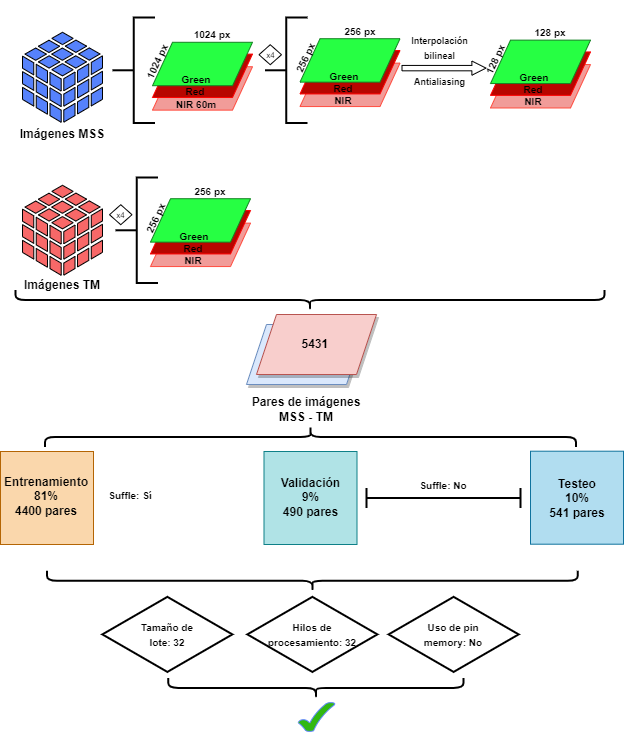
\includegraphics[width=1\linewidth]{2_CAPITULO4/IMG/dataloader.png}
                    \begin{justify}
                        \textit{Nota.} El gráfico detalla el flujo de datos en la preparación de imágenes satelitales MSS y TM, su segmentación en lotes y la configuración eficiente de dataloaders para el modelo.
                    \end{justify}                    
                    \label{dataloader}
                \end{figure}

                Este proceso no solo facilita el manejo eficiente de los datos, sino que también asegura que cada par de imágenes MSS y TM sea procesado y presentado al modelo de manera óptima, mejorando la precisión y efectividad del entrenamiento para la armonización de bandas.



        \subsection{Desarrollo del modelo MSS2TM}


        
            \subsubsection{Configuración del entorno de trabajo}
                Se estableció un entorno de trabajo en Python mediante la creación de un entorno virtual utilizando herramientas como entornos de conda. Esto permitió una separación clara y la gestión de dependencias específicas del proyecto. Se instaló PyTorch, seleccionando una versión que correspondiera a la compatibilidad con CUDA del sistema utilizado, para facilitar el entrenamiento acelerado por GPU.
            
                Además, se implementaron herramientas de registro y monitoreo para seguir el progreso del entrenamiento y se estableció un sistema de control de versiones para el código y los datos. La automatización y orquestación del flujo de trabajo, junto con la validación del código mediante pruebas unitarias y de integración, formaron parte esencial de este proceso. Todas las dependencias se documentaron en un archivo requirements.txt para facilitar la configuración reproducible del entorno.


            \subsubsection{Elección de arquitecturas para el generador y discriminador en GANs}
                En la fase de desarrollo del modelo se escogió con detenimiento la arquitectura para cada componente de la Red Neuronal Generativa Adversaria (GAN), fundamental para la consecución de nuestros objetivos. El generador, implementado como un Transformer Visual, conocido comúnmente por su acrónimo en inglés VIT (Vision Transformer), fue diseñado para procesar y transformar imágenes de múltiples espectros (MSS) en imágenes de alta resolución (HR) o TM. Esta elección se basó en la capacidad de los Transformers Visuales para manejar secuencias de datos, lo que resulta ideal para comprender y generar representaciones complejas de imágenes. Por otro lado, para el discriminador, se optó por una arquitectura de Perceptrón Multicapa (MLP), que debido a su simplicidad y eficacia en tareas de clasificación, resultó ser la más adecuada para evaluar la autenticidad de las imágenes generadas por el VIT, diferenciando entre las reales y las producidas artificialmente. 
            
         
                \begin{figure}[H] 
                    \caption{\doublespacing \\ \textit{Arquitectura de Super-Resolución para armonización de imágenes Landsat MSS y TM utilizando SWINIR.}} 
                    \centering
                    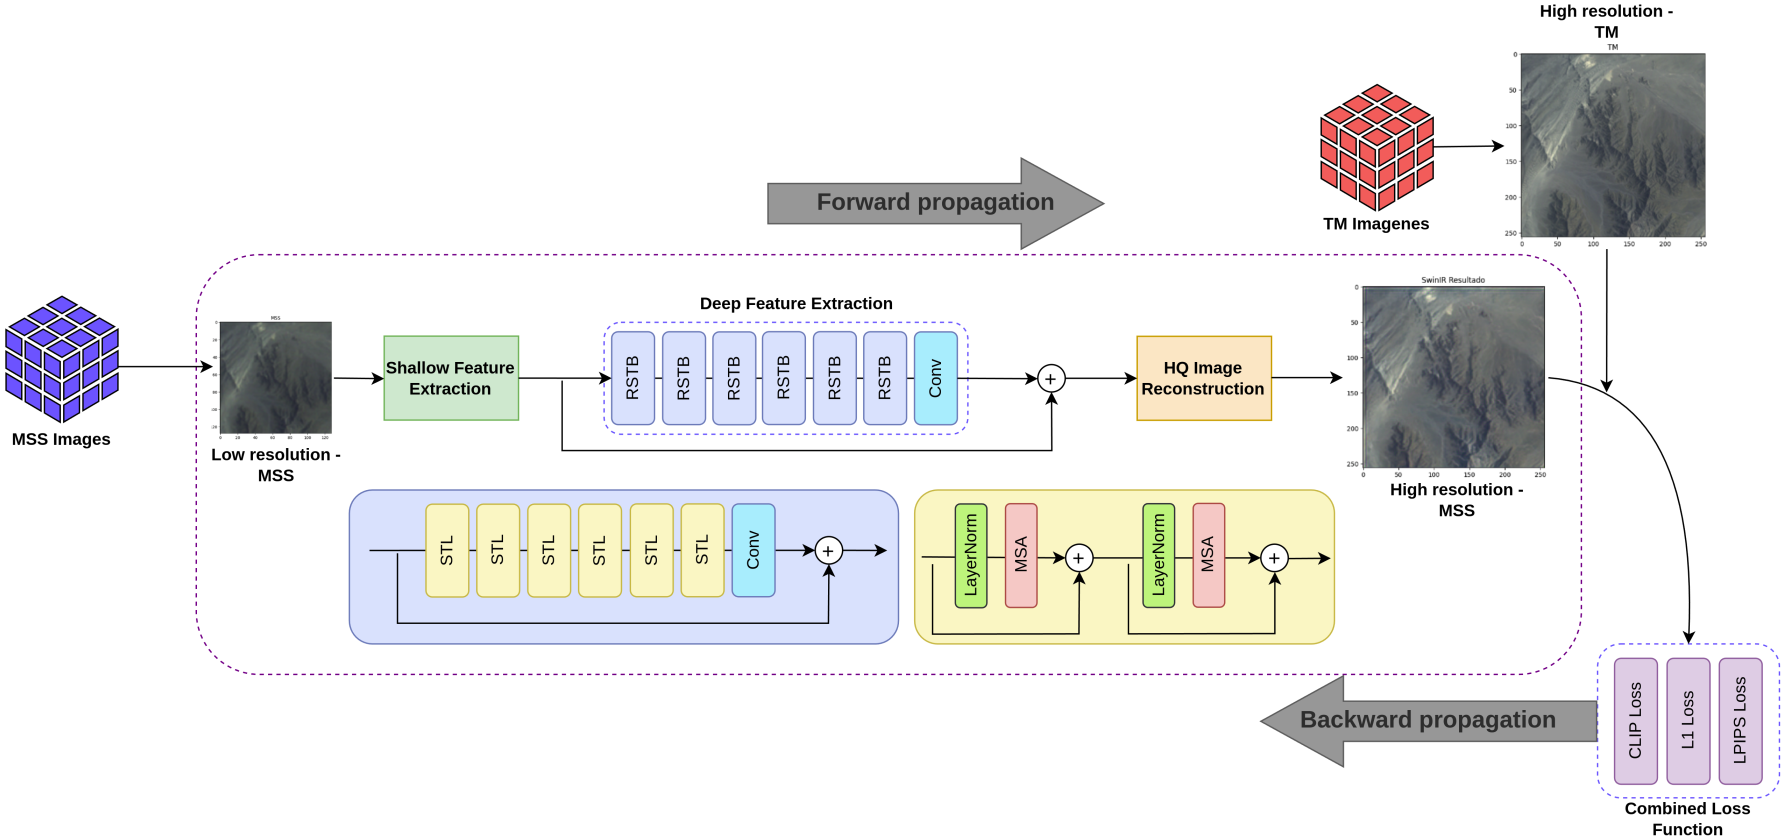
\includegraphics[width=1\linewidth]{2_CAPITULO4/IMG/SWINIR.png}
                    \begin{justify}
                        \textit{Nota.} El diagrama muestra el proceso de extracción y reconstrucción de características para convertir imágenes de baja resolución MSS en alta resolución utilizando SWINIR, integrando módulos RSTB y STL para mejorar la calidad de las imágenes resultantes.
                    \end{justify}                    
                    \label{generador}
                \end{figure}
    

                \begin{figure}[H] 
                    \caption{\doublespacing \\ \textit{Flujo del discriminador MLP.}} 
                    \centering
                    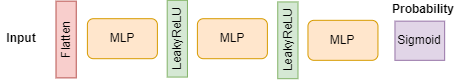
\includegraphics[width=0.6\linewidth]{2_CAPITULO5/IMG/mlp_discriminator.png}
                    \begin{justify}
                        \textit{Nota.} Se muestra un flujo del discriminador MLP inicia con entrada de imagen, pasa por capas MLP y Leaky ReLU, culmina con probabilidad sigmoide.
                    \end{justify}                    
                    \label{discriminador}
                \end{figure}

            \subsubsection{Definición de parámetros y funciones de pérdida}
                Se definieron las funciones de pérdida para entrenar el modelo. El L1 Loss se utilizó para minimizar la diferencia absoluta píxel por píxel entre las imágenes generadas por el modelo (\(TM_{hat}\)) y las imágenes objetivo (TM), con el fin de asegurar una alta fidelidad visual. Además, se implementó una función de pérdida adicional para el discriminador, donde se estimó la probabilidad de que una imagen sea real o falsa (L2), promoviendo la generación de imágenes que el discriminador no pudiera distinguir de las reales.

            \subsubsection{Proceso de entrenamiento}
                En la fase de entrenamiento, se ajustaron los parámetros de los modelos generador y discriminador de manera iterativa. Se comenzó con una tasa de aprendizaje adaptativa y un coeficiente \( \alpha \) inicialmente establecido en 0.5 para equilibrar las funciones de pérdida L1 y L2. Tras experimentación empírica, se estableció que un \( \alpha \) de 0.01 proporcionaba un equilibrio más efectivo, reduciendo las distorsiones en las imágenes generadas y mejorando la estabilidad del entrenamiento. La optimización se llevó a cabo utilizando el algoritmo Adam, y se incorporó la técnica de dropout para prevenir el sobreajuste. A lo largo del proceso, la pérdida observada disminuyó de manera sostenida, lo que indicó una mejora continua en la precisión del modelo. Además, se emplearon técnicas de aumento de datos y selección aleatoria de lotes para fortalecer la robustez del entrenamiento.

                Durante esta fase, también se enfatizó la importancia de una inicialización adecuada y un registro detallado del proceso. Se utilizó PyTorch por su eficiencia y flexibilidad, configurando aspectos fundamentales como la semilla aleatoria y el dispositivo de cálculo para asegurar un entrenamiento estable y reproducible. Herramientas de registro como Weights and Biases (wandb) permitieron monitorear en tiempo real métricas clave como la pérdida y la precisión, facilitando un seguimiento detallado del entrenamiento.

                La carga de datos se optimizó mediante la biblioteca ML-STAC, lo que garantizó una gestión eficiente de los grandes conjuntos de datos de imágenes satelitales. Este enfoque uniformó la carga de datos y mejoró la integración de los mismos en el entrenamiento.

                El cálculo de métricas específicas como la pérdida L1, la pérdida perceptual y la pérdida GAN proporcionó información valiosa sobre el rendimiento del modelo, ayudando en la afinación y el ajuste de hiperparámetros. La implementación de un sistema de checkpointing aseguró la recuperación del entrenamiento en caso de interrupciones, facilitando la experimentación con diferentes configuraciones y el almacenamiento periódico de los estados del modelo, la configuración del optimizador y otros hiperparámetros.

            \subsubsection{Ajuste y optimización}
                El proceso de ajuste fino del modelo, que comprende tanto el generador, implementado con la arquitectura VIT, como el discriminador, basado en un MLP, fue crucial para lograr resultados satisfactorios. Durante esta etapa, se experimentó con variaciones en los hiperparámetros y se aplicó la validación cruzada para asegurar la generalización del modelo. Para el discriminador, se desarrolló una estrategia de entrenamiento que moderaba la actualización de sus parámetros, buscando mantener el equilibrio de Nash y evitar el colapso del modelo. Este cuidadoso ajuste se extendió al generador, donde se aplicaron técnicas como la corrección de máscaras basada en cuantiles y operaciones de división o sustracción, permitiendo refinar la representación de las imágenes generadas. Se emplearon tanto el \(L1\) Loss, para minimizar la diferencia absoluta píxel por píxel entre las imágenes generadas y las de referencia, asegurando así una alta fidelidad visual, como el \(L2\) Loss, para evaluar la capacidad del generador de producir imágenes que el discriminador considere reales. La combinación de estas estrategias resultó en una notable mejora en la precisión, fidelidad y realismo de las imágenes generadas, validando la eficacia de las arquitecturas y metodologías de entrenamiento empleadas.

            
                \subsubsection{Configuración de las funciones de pérdida}
                    La eficacia de un modelo de superresolución como MSS2TM depende en gran medida de las funciones de pérdida utilizadas durante el entrenamiento. Estas funciones de pérdida son cruciales para guiar el proceso de aprendizaje del modelo hacia la generación de imágenes que no solo son visualmente atractivas, sino que también son fieles a las características reales de las imágenes de alta resolución. Para el modelo MSS2TM, se adoptó un enfoque multiobjetivo en la selección y configuración de las funciones de pérdida, basándose en la naturaleza de las imágenes MSS y TM.
                
                    \paragraph{CLIP Loss}
                        La función de pérdida CLIP (Contrastive Language-Image Pretraining) Loss se emplea para asegurar que las imágenes generadas sean coherentes con las características contextuales y semánticas aprendidas a partir de grandes conjuntos de datos de imágenes y texto. CLIP Loss utiliza un modelo preentrenado que compara las imágenes generadas con descripciones textuales, asegurando que las imágenes producidas no solo sean visualmente similares, sino que también mantengan una coherencia semántica con las descripciones esperadas.

                    \paragraph{L1 Loss}
                        El L1 Loss, también conocido como L1-norm loss o Mean Absolute Error (MAE), mide la diferencia absoluta entre los valores de los píxeles de la imagen generada y la imagen de referencia. Esta función de pérdida es esencial para asegurar que las imágenes generadas sean lo más similares posible a las imágenes de alta resolución en términos de detalles y texturas finas.

                    \paragraph{LPIPS Loss}
                        La función de pérdida LPIPS (Learned Perceptual Image Patch Similarity) se utilizó para evaluar la similitud perceptual entre las imágenes generadas y las de alta resolución. LPIPS aprovecha un modelo preentrenado para comparar las características visuales y contextuales de las imágenes. Esta función de pérdida es particularmente efectiva para asegurar que las imágenes superresueltas no solo coincidan en términos de píxeles, sino que también capturen con precisión los elementos y patrones semánticos presentes en las imágenes TM de alta resolución.

                    \begin{figure}[H] 
                        \caption{\doublespacing \\ \textit{Flujo  de la arquitectura GAN - MSS2TM para la armonización espectral y espacial.}} 
                        \centering
                        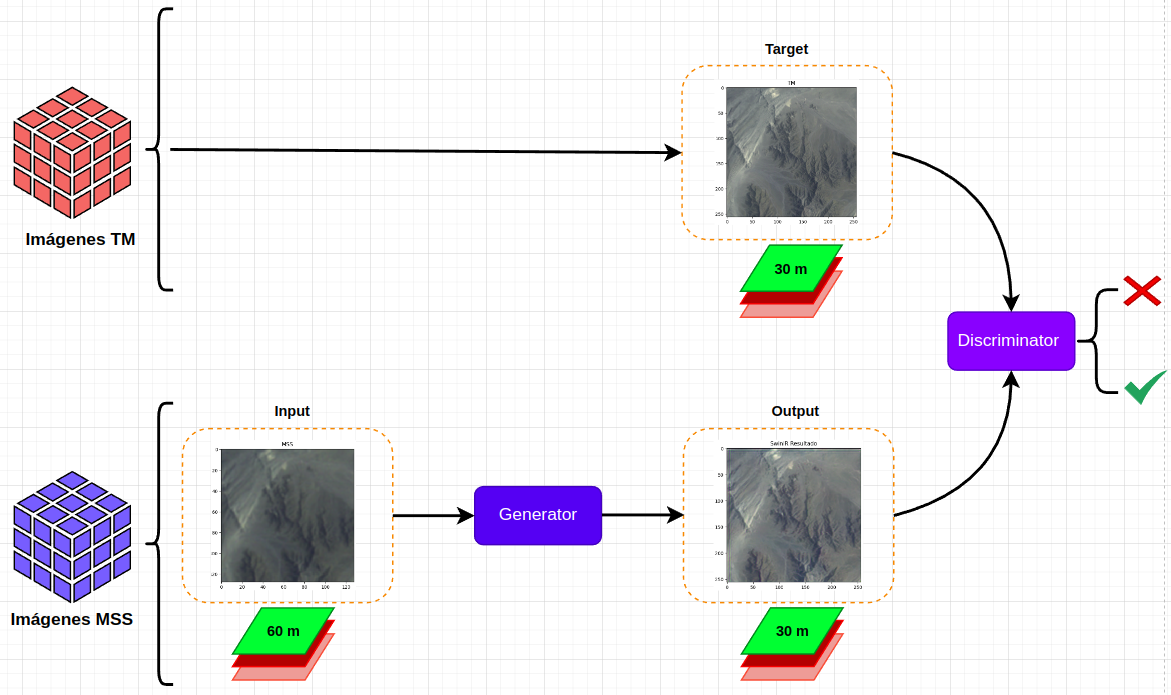
\includegraphics[width=1\linewidth]{2_CAPITULO4/IMG/GAN.png}
                        \begin{justify}
                            \textit{Nota.} El diagrama ilustra el flujo de trabajo de una arquitectura GAN para transformar imágenes MSS de 60m a una resolución de 30m, evaluadas por un discriminador para mejorar la armonización espectral y espacial​.
                        \end{justify}                    
                        \label{gan}
                    \end{figure}

        \subsection{Generación de bandas virtuales en imágenes MSS}
            Una vez que las imágenes MSS se alinean espectral y espacialmente con las TM gracias al modelo MSS2TM, el siguiente paso es generar bandas sintéticas o virtuales para las MSS que existen en las TM pero no en las MSS. 
            
            \subsubsection{Adquisición y procesamiento inicial de datos}
                Se comenzó con reconocer el sistema multiespectral MSS, que contenían bandas espectrales en el rango del infrarrojo cercano (NIR), rojo y verde, todas con una resolución de 30 metros.

            \subsubsection{Entrenamiento del perceptrón multicapa (MLP)}
                El diseño y entrenamiento de un MLP constituyó el núcleo del enfoque adoptado para predecir las bandas espectrales faltantes en las imágenes MSS. La red neuronal profunda se estructuró mediante la inclusión de capas lineales y una arquitectura que promovió el aprendizaje de patrones complejos por medio de activaciones no lineales y la regulación de conexiones entre neuronas. El propósito fue refinar los parámetros del modelo de manera que este pudiera replicar con exactitud las bandas adicionales necesarias, simulando efectivamente una imagen TM completa.

                La implementación del modelo MLP se realizó extendiendo la clase Module de PyTorch, integrando tres capas lineales (nn.Linear) intercaladas con funciones de activación no lineales (nn.ReLU) y una capa de abandono (nn.Dropout) para la regularización. La configuración de la red permitió la transformación de la entrada a un espacio de características ocultas, seguido por el procesamiento intermedio de estas características, y finalmente, su conversión al espacio de salida deseado mediante la última capa lineal. La inclusión de la función de activación ReLU facilitó el aprendizaje de relaciones complejas entre las entradas y las salidas, mientras que la capa de abandono contribuyó a la prevención del sobreajuste mediante el descarte aleatorio de algunas características durante el entrenamiento.
                
                La lógica de procesamiento de datos se definió en la función forward, asegurando el paso secuencial de los datos a través de las capas lineales, la activación ReLU y el abandono, antes de emitir la salida final.
                
                El entrenamiento del modelo se organizó a través de la función \texttt{run\_deep\_prior}, que inició con la preparación de los datos de entrada y salida en un formato adecuado. Posteriormente, se instanció el modelo MLP, configurando el optimizador Adam y la función de pérdida L1, esenciales para el proceso de aprendizaje.

            \subsubsection{Proceso de entrenamiento y ajuste fino}
                El modelo se sometió a un régimen de entrenamiento iterativo y exhaustivo, durante el cual se realizaron actualizaciones graduales y precisas en la configuración interna de la red. Se emplearon lotes de datos pequeños para optimizar los recursos computacionales y mejorar la capacidad del modelo para generalizar a partir de los datos proporcionados. La estrategia de entrenamiento estuvo guiada por un enfoque de minimización de errores, donde se buscaba reducir la diferencia entre las bandas espectrales conocidas y las predicciones del modelo.

                \paragraph{Histograma matching}
                    El \textit{histograma matching} se utiliza para normalizar los valores de reflectancia entre diferentes imágenes. Este proceso implica corregir los histogramas de las imágenes para que tengan una distribución similar, lo cual es crucial para mantener la coherencia en las bandas generadas.

                \paragraph{Normalización de valores de reflectancia}
                    El modelo también intenta normalizar los valores de reflectancia. Este proceso es complicado debido a que las mismas bandas de diferentes imágenes pueden tener distintos valores de reflectancia. La normalización correcta es esencial para obtener resultados precisos en la generación de imágenes de mayor resolución.

                \paragraph{Modelos con diferentes parámetros}
                    La comparación entre modelos con distintos números de parámetros (por ejemplo, 68 vs. 128 parámetros) es importante para evaluar el impacto en el rendimiento y la precisión de la superresolución. Además, fue crucial encontrar el número adecuado de iteraciones (por ejemplo, 2000 pasos) para entrenar el modelo, lo cual puede variar debido a la aleatoriedad en el entrenamiento.

                \paragraph{Early stopping}
                    Implementar \textit{early stopping} fue una estrategia eficaz para detener el entrenamiento del modelo una vez que alcanza una meseta en su rendimiento. Esto evitó el sobreentrenamiento y mejora la eficiencia del modelo, permitiendo un uso óptimo de los recursos computacionales.

                \paragraph{Mantener la firma espectral}
                    La preservación de la forma de la firma espectral fue crucial para asegurar la precisión en la generación de bandas. No solo fue importante mantener los valores de intensidad, sino también la forma de la firma espectral. Esto pudo requerir ajustar los parámetros del modelo, aumentando su complejidad para mantener la integridad espectral.


            \begin{figure}[H] 
                \caption{\doublespacing \\ \textit{Modelo de armonización para imágenes Landsat MSS.}} 
                \centering
                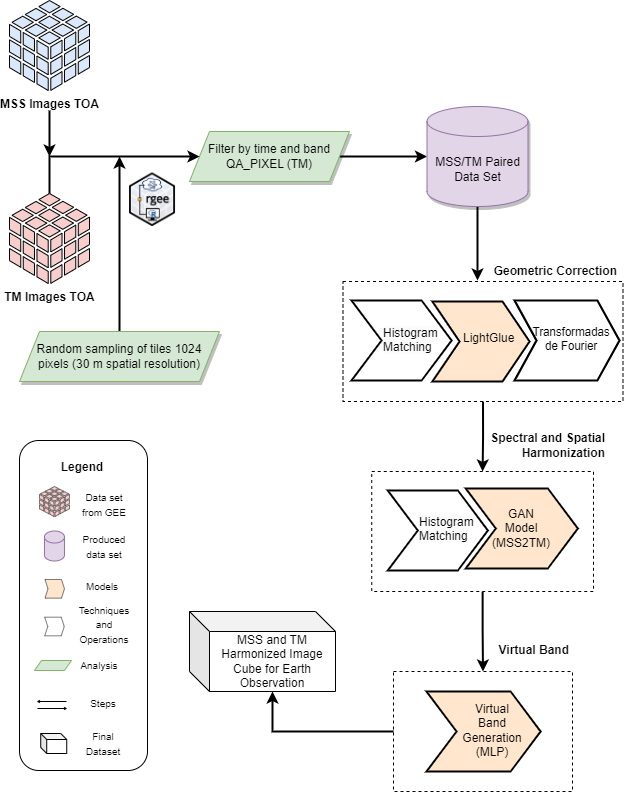
\includegraphics[width=0.95\linewidth]{2_CAPITULO5/IMG/modelo.png}
                \begin{justify}
                    \textit{Nota.} El esquema presenta una metodología de armonización de imágenes de sensores MSS y TM: comienza con imágenes TOA, sigue con correcciones geométricas y transformadas de Fourier via LightGlue, continúa con armonización espectral y espacial mediante una arquitectura GAN y culmina con un cubo de imagen armonizado para la creación de bandas virtuales.
                \end{justify}                    
                \label{modelo2}
            \end{figure}

    \section{Análisis estadístico}

        En la fase de preparación para la validación de los modelos desarrollados, se diseñó un enfoque de análisis estadístico detallado. Este diseño metodológico fue crucial para asegurar que, una vez aplicados, los modelos pudieran demostrar un ajuste adecuado a los datos de entrenamiento y una generalización efectiva a nuevos conjuntos de datos.
            
        \subsection{Validación cuantitativa}
            
            Se emplearon las siguientes métricas para evaluar el desempeño del modelo:
            
            \subsubsection{Error Absoluto Medio (MAE)} 
                Esta métrica midió la diferencia media absoluta entre los valores predichos por el modelo y los valores reales. Fue útil para entender el error promedio por píxel en las imágenes generadas.
                
            \subsubsection{Raíz del Error Cuadrático Medio (RMSE)} 
                Similar al MAE, pero penalizó más los errores grandes, ofreciendo una visión más estricta de la precisión del modelo.
                
            \subsubsection{Coeficiente de Correlación de Pearson (R)} 
                Midió la relación lineal entre los valores predichos y los valores reales, proporcionando una medida de cuán bien las predicciones siguieron las tendencias reales.
            
        \subsection{Evaluación de métricas de rendimiento}
            
            Para asegurar que las imágenes generadas no solo coincidieran en términos de píxeles, sino que también capturaran con precisión los elementos y patrones semánticos presentes en las imágenes TM de alta resolución, se utilizaron las siguientes funciones de pérdida:
            
            \subsubsection{CLIP Loss} 
                Se empleó para asegurar que las imágenes generadas fueran coherentes con las características contextuales y semánticas aprendidas a partir de grandes conjuntos de datos de imágenes y texto. Utilizó un modelo preentrenado que comparaba las imágenes generadas con descripciones textuales.
                
            \subsubsection{L1 Loss} 
                También conocido como Mean Absolute Error (MAE), midió la diferencia absoluta entre los valores de los píxeles de la imagen generada y la imagen de referencia. Fue esencial para asegurar que las imágenes generadas fueran lo más similares posible a las imágenes de alta resolución en términos de detalles y texturas finas.
                
            \subsubsection{LPIPS (Learned Perceptual Image Patch Similarity) Loss} 
                Evaluó la similitud perceptual entre las imágenes generadas y las de alta resolución. Aprovechó un modelo preentrenado para comparar las características visuales y contextuales de las imágenes, asegurando que las imágenes superresueltas capturaran con precisión los elementos y patrones semánticos presentes en las imágenes TM de alta resolución.
                